This section outlines the InternHub – Students \& Companies (S\&C) platform's user interface, including a summary of the main pages that make up the system. Since changes to the design may be made throughout the testing phase, the design mockups displayed here focus more on the interface's usability and interaction dynamics than on its final visual aesthetics. Equivalent pages will be made for mobile devices, even if the desktop browser version is the main focus due to its suitability for thorough profile management and internship-related procedures. By adapting and scaling the interface to fit smaller screens, this guarantees a seamless user experience.

The design prototypes shown here serve as a fundamental depiction of the platform's user interface, as specified in the RASD. As the system develops, these designs are subject to optimization and improvement, taking into account input from user interactions and testing.

\section{Overview}
\label{sec:overview}%
\begin{figure}[H]
    \begin{center}
        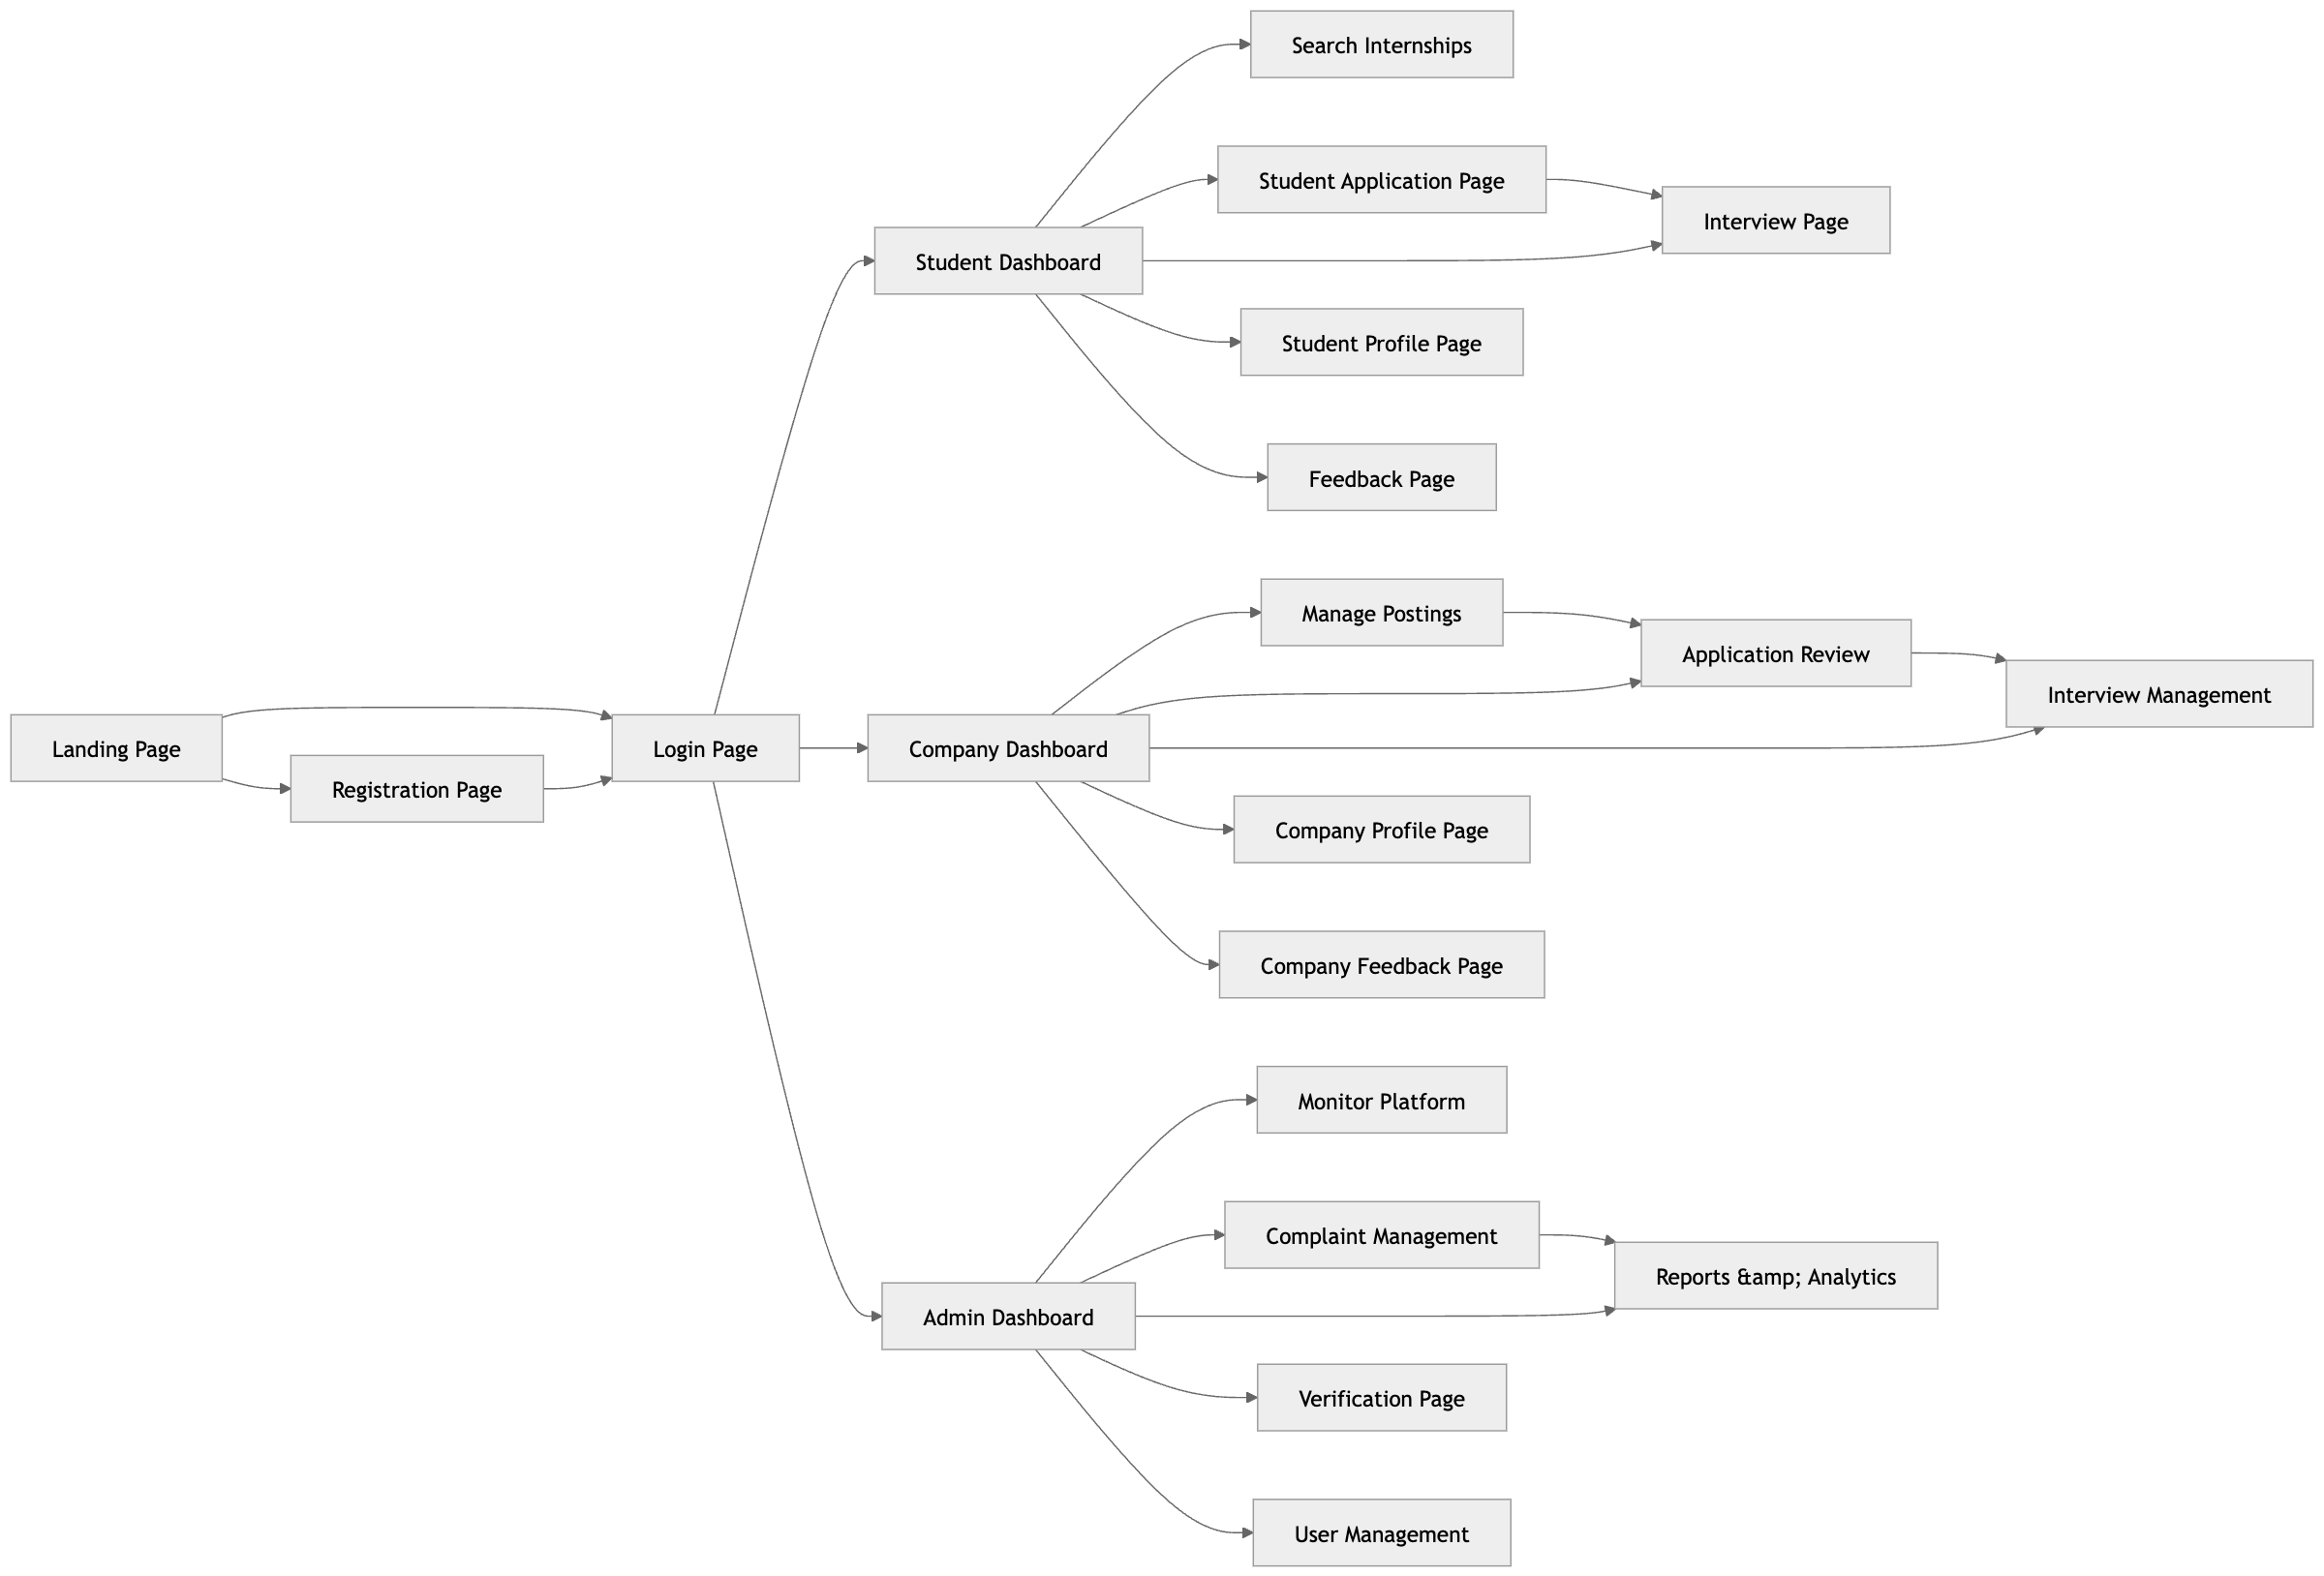
\includegraphics[width=0.82\linewidth]{JhaBhatiaSharma/imagesDD/UIOverview.png}
        \caption{UI Overview}
        \label{fig:uiOverview}
    \end{center}
\end{figure}

This graphic shows the flow and relationships between distinct pages designed for different user roles, giving a thorough overview of the InternHub – Students \& Companies (S\&C) platform's user interface (UI) architecture. 

\begin{enumerate}
    \item \textbf{Landing Page:} Directs users to either the Registration Page for new users or the Login Page for existing users.
    \item \textbf{Role-Specific Dashboards:}
    \begin{itemize}
        \item \textbf{Student Dashboard:} Access to Search Internships, Student Application Page, Feedback Page, Student Profile Page, and Interview Management.
        \item \textbf{Company Dashboard:} Supports recruitment workflows, providing access to the Company Profile Page, Feedback Page, and tools for managing postings and reviewing applications.
        \item \textbf{Admin Dashboard:} Enables administrative oversight with features like User Management, Complaint Management, Verification Page, and Reports \& Analytics.
    \end{itemize}
\end{enumerate}

This structured design emphasizes role-specific features and smooth navigation, ensuring an effective user experience for all stakeholders. The diagram's links illustrate the dynamic and scalable nature of the interface, tailored to the diverse needs of administrators, businesses, and students.

\section{User Interfaces}
\label{sec:user_interfaces}%

\subsection{UI1. Login}
\label{subsec:login_ui}%
\begin{figure}[H]
    \begin{center}
        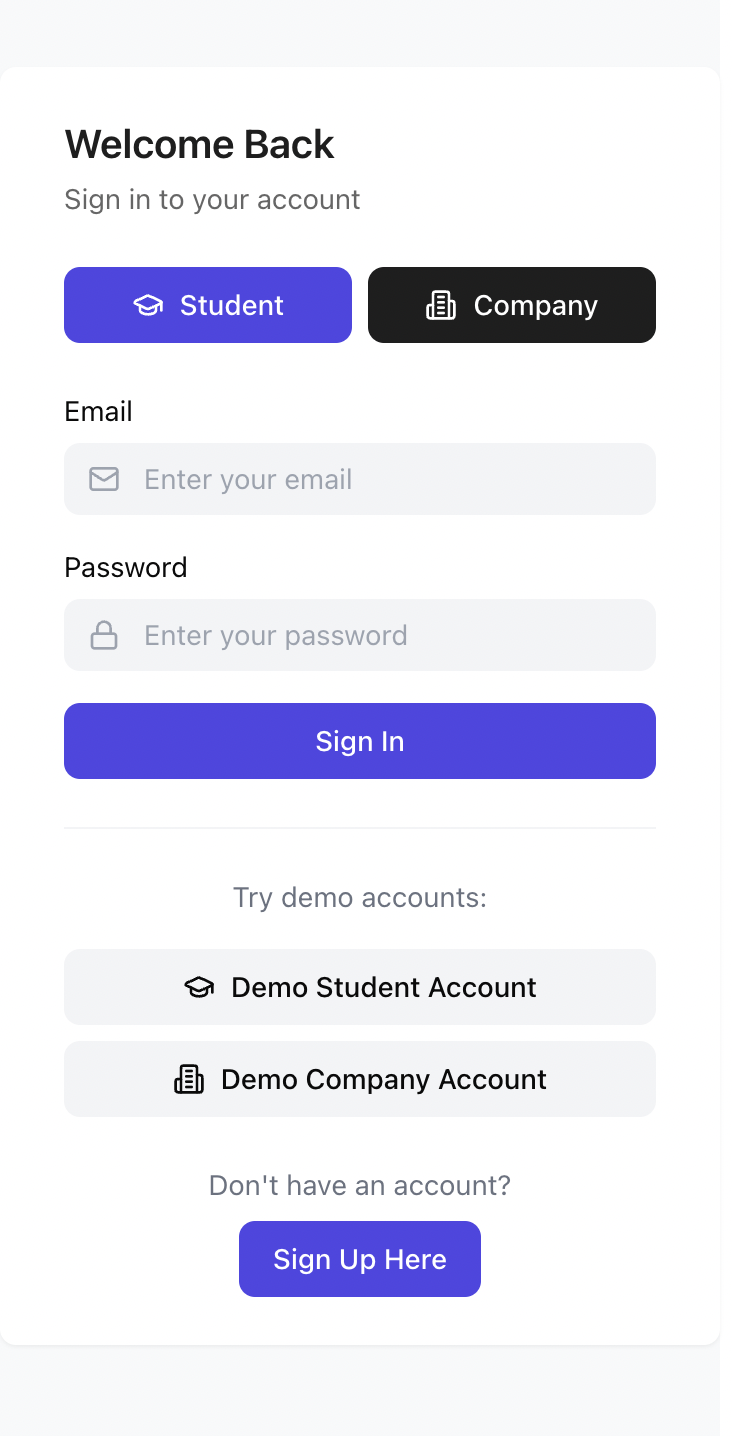
\includegraphics[width=0.52\linewidth]{JhaBhatiaSharma/imagesDD/LoginMockup.png}
        \caption{Login Interface Mockup}
        \label{fig:LoginInterface}
    \end{center}
\end{figure}
The login page is designed to provide a seamless access experience for the two main user roles: companies and students. 

\begin{enumerate}
    \item \textbf{Role Toggle:} A toggle option at the top allows users to select their role, ensuring a tailored login experience.
    \item \textbf{User Input Fields:} Users input their email and password, supported by intuitive placeholders.
    \item \textbf{"Sign In" Button:} Prominently displayed for easy access.
    \item \textbf{Demo Accounts:} Allows users to test features without signing up.
    \item \textbf{"Sign Up Here" Link:} Redirects new users to the registration page.
\end{enumerate}

The simple, clear design ensures an intuitive experience for all users while maintaining a professional appearance.

\subsection{UI2. SignUp}
\label{subsec:signup_ui}%

\begin{figure}[H]
    \begin{center}
        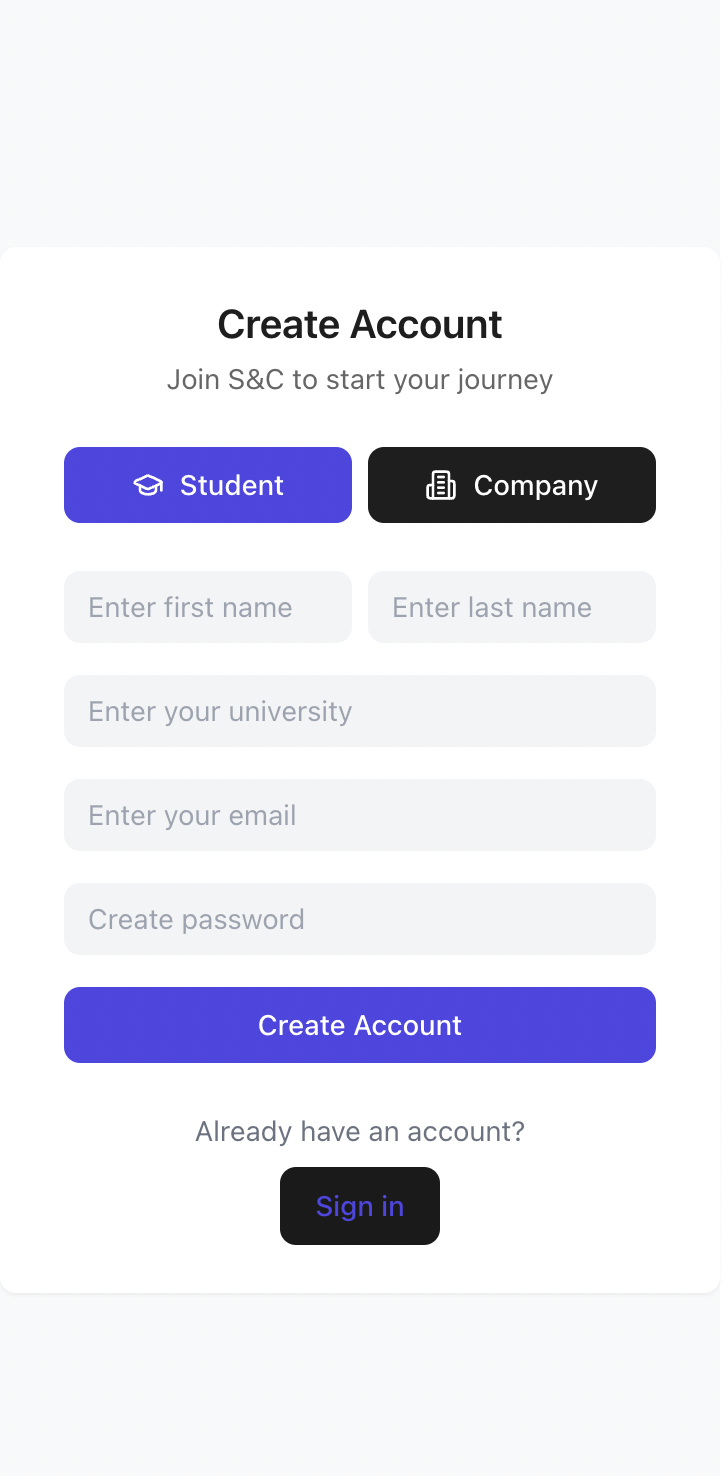
\includegraphics[width=0.52\linewidth]{JhaBhatiaSharma/imagesDD/SignUp.png}
        \caption{SignUp Interface Mockup}
        \label{fig:signupinterface}
    \end{center}
\end{figure}

The registration page provides a streamlined and user-friendly interface for new users to create accounts.

\begin{enumerate}
    \item \textbf{Role Selection:} Users can switch between Student and Company roles at the top of the page.
    \item \textbf{Input Fields:} Includes First Name, Last Name, University (for students), Email, and Password.
    \item \textbf{"Create Account" Button:} Simplifies the submission process.
    \item \textbf{"Sign In" Link:} Redirects existing users to the login page.
\end{enumerate}

This design guarantees a professional and user-friendly experience for new users entering the platform.

\subsection{UI3. Company Dashboard}
\label{subsec:company_dashboard_ui}%

\begin{figure}[H]
    \begin{center}
        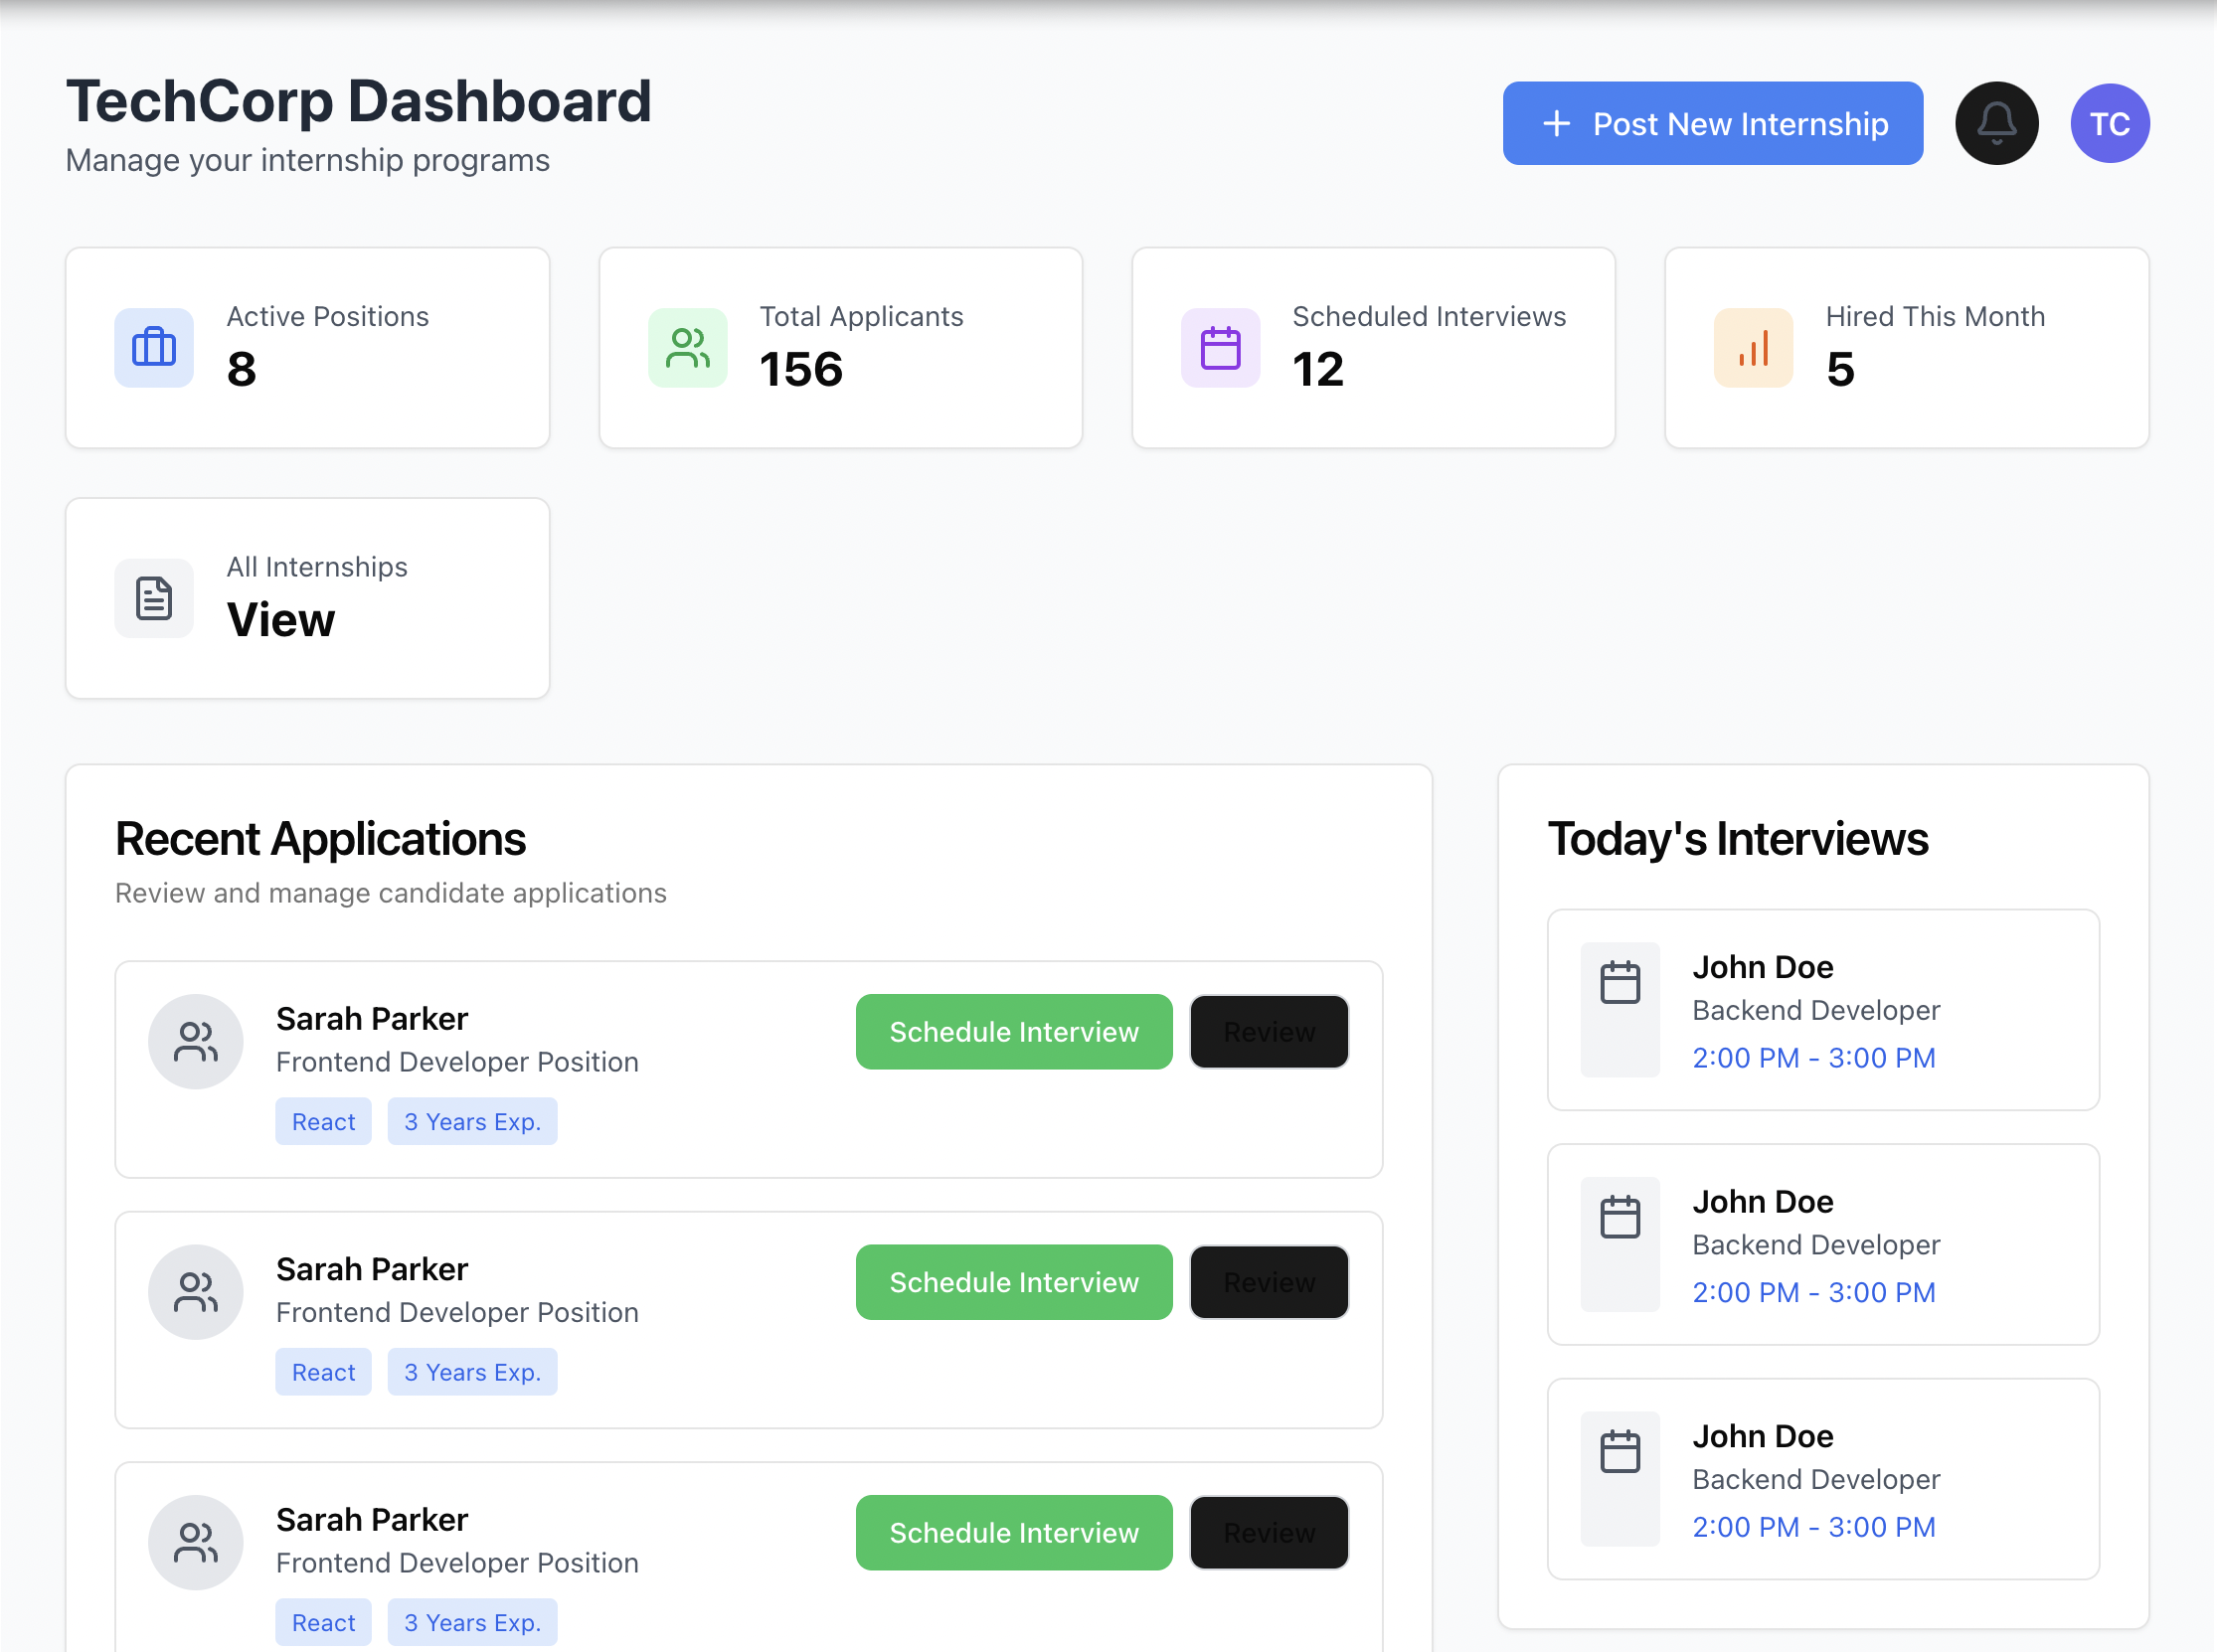
\includegraphics[width=0.82\linewidth]{JhaBhatiaSharma/imagesDD/CompanyDashboard.png}
        \caption{Company Dashboard}
        \label{fig:companyDashboard}
    \end{center}
\end{figure}

The Company Dashboard offers a well-structured interface for recruiters to efficiently manage their internship programs.

\begin{enumerate}
    \item \textbf{Dashboard Overview:} Displays key metrics such as Active Positions, Total Applicants, Scheduled Interviews, and Hired This Month.
    \item \textbf{Post Internship:} A quick-access button for creating new internship postings.
    \item \textbf{Recent Applications:} Displays candidate submissions with relevant details like name, position applied for, skills, and experience. Includes options to schedule interviews or review applications.
    \item \textbf{Today's Interviews:} Shows a compact schedule of interviews, including candidate names, positions, and times.
\end{enumerate}

This layout ensures all essential information is easily accessible, enabling recruiters to navigate and complete their tasks effectively.

\subsection{UI4. Post Internship}
\label{subsec:post_internship_ui}%

\begin{figure}[H]
    \begin{center}
        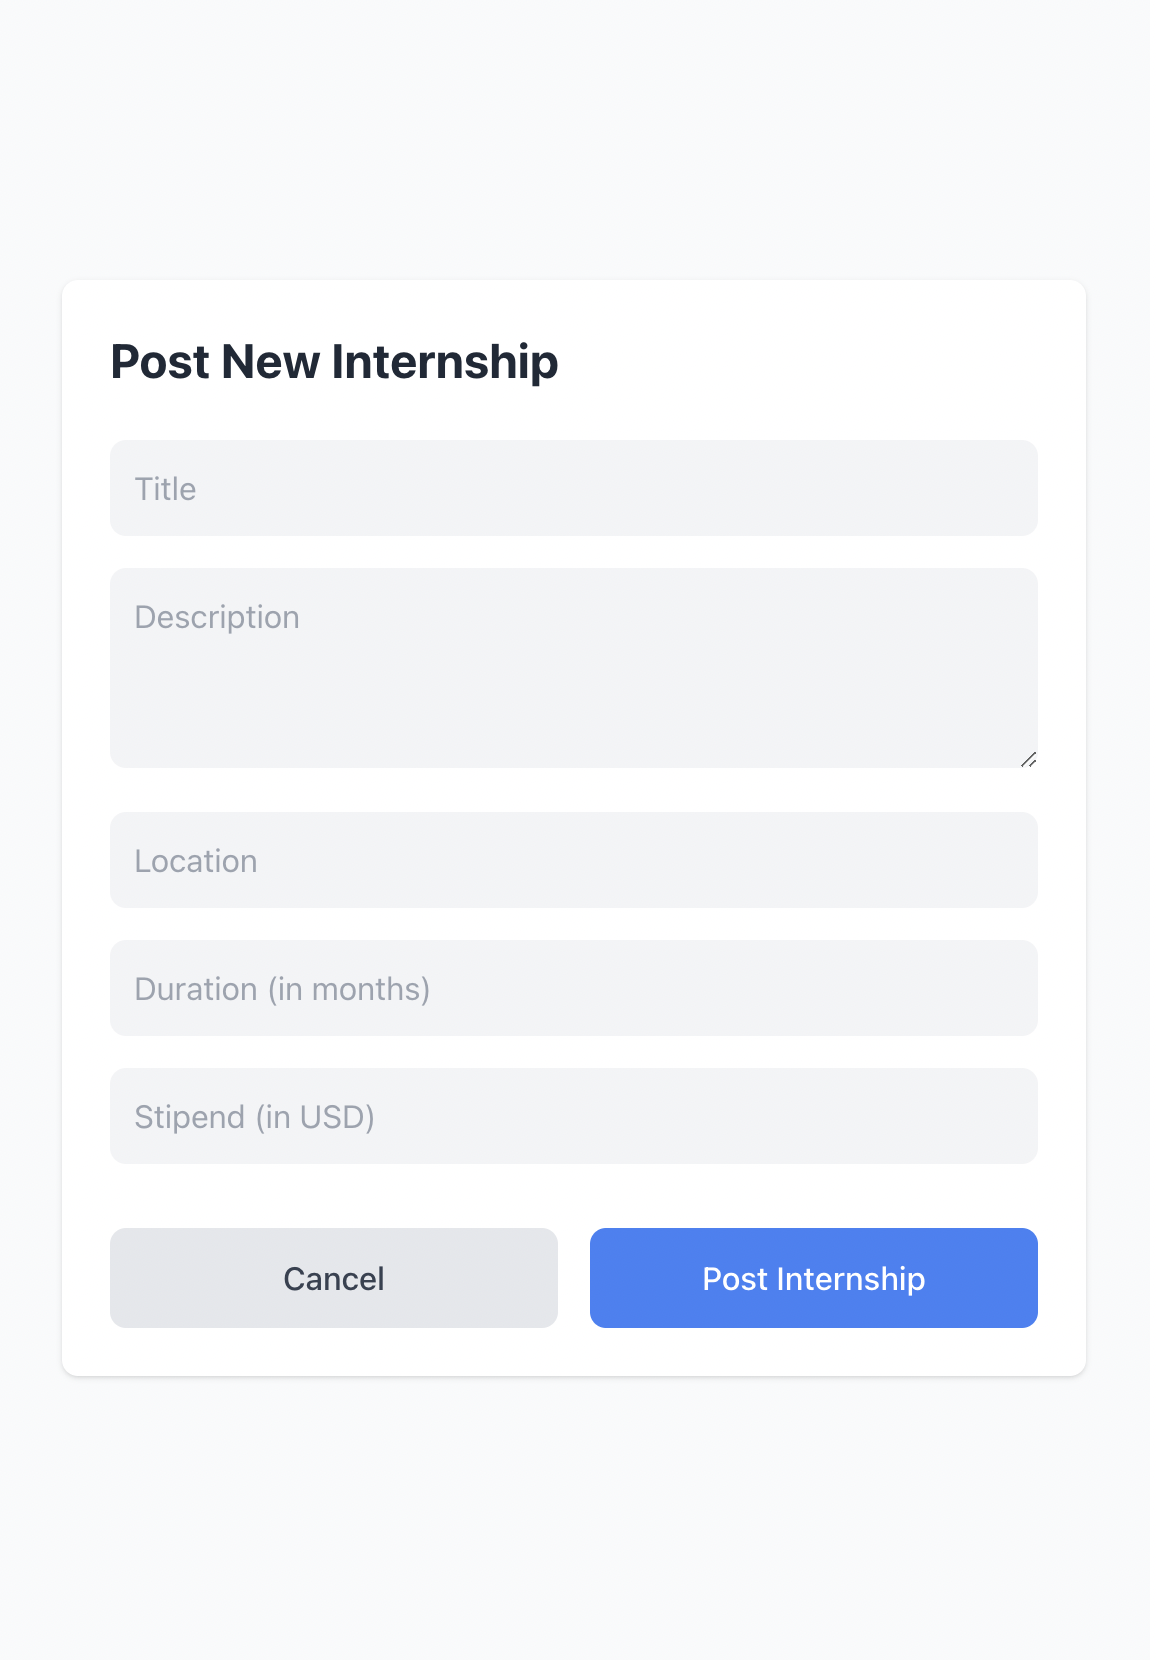
\includegraphics[width=0.62\linewidth]{JhaBhatiaSharma/imagesDD/PostInternship.png}
        \caption{Post Internship}
        \label{fig:postInternship}
    \end{center}
\end{figure}

Recruiters can post internship opportunities to the platform using a structured interface by utilizing the \textbf{Post New Internship} form. The form includes fields for essential details such as:
\begin{enumerate}
    \item \textbf{Title:} The name of the internship position.
    \item \textbf{Description:} Detailed information about the role and responsibilities.
    \item \textbf{Location:} The physical or remote location of the internship.
    \item \textbf{Duration:} Length of the internship in months.
    \item \textbf{Stipend:} Information about the compensation provided.
\end{enumerate}

The form is designed with clearly defined and spaced fields to ensure clarity and ease of use. At the bottom, a \textbf{Post Internship} button enables submission of the internship details, while a \textbf{Cancel} button allows recruiters to terminate the process. This arrangement prioritizes simplicity and functionality, enabling businesses to efficiently communicate openings to prospective candidates.

\subsection{UI5. Student Dashboard}
\label{subsec:student_dashboard_ui}%
\begin{figure}[H]
    \begin{center}
        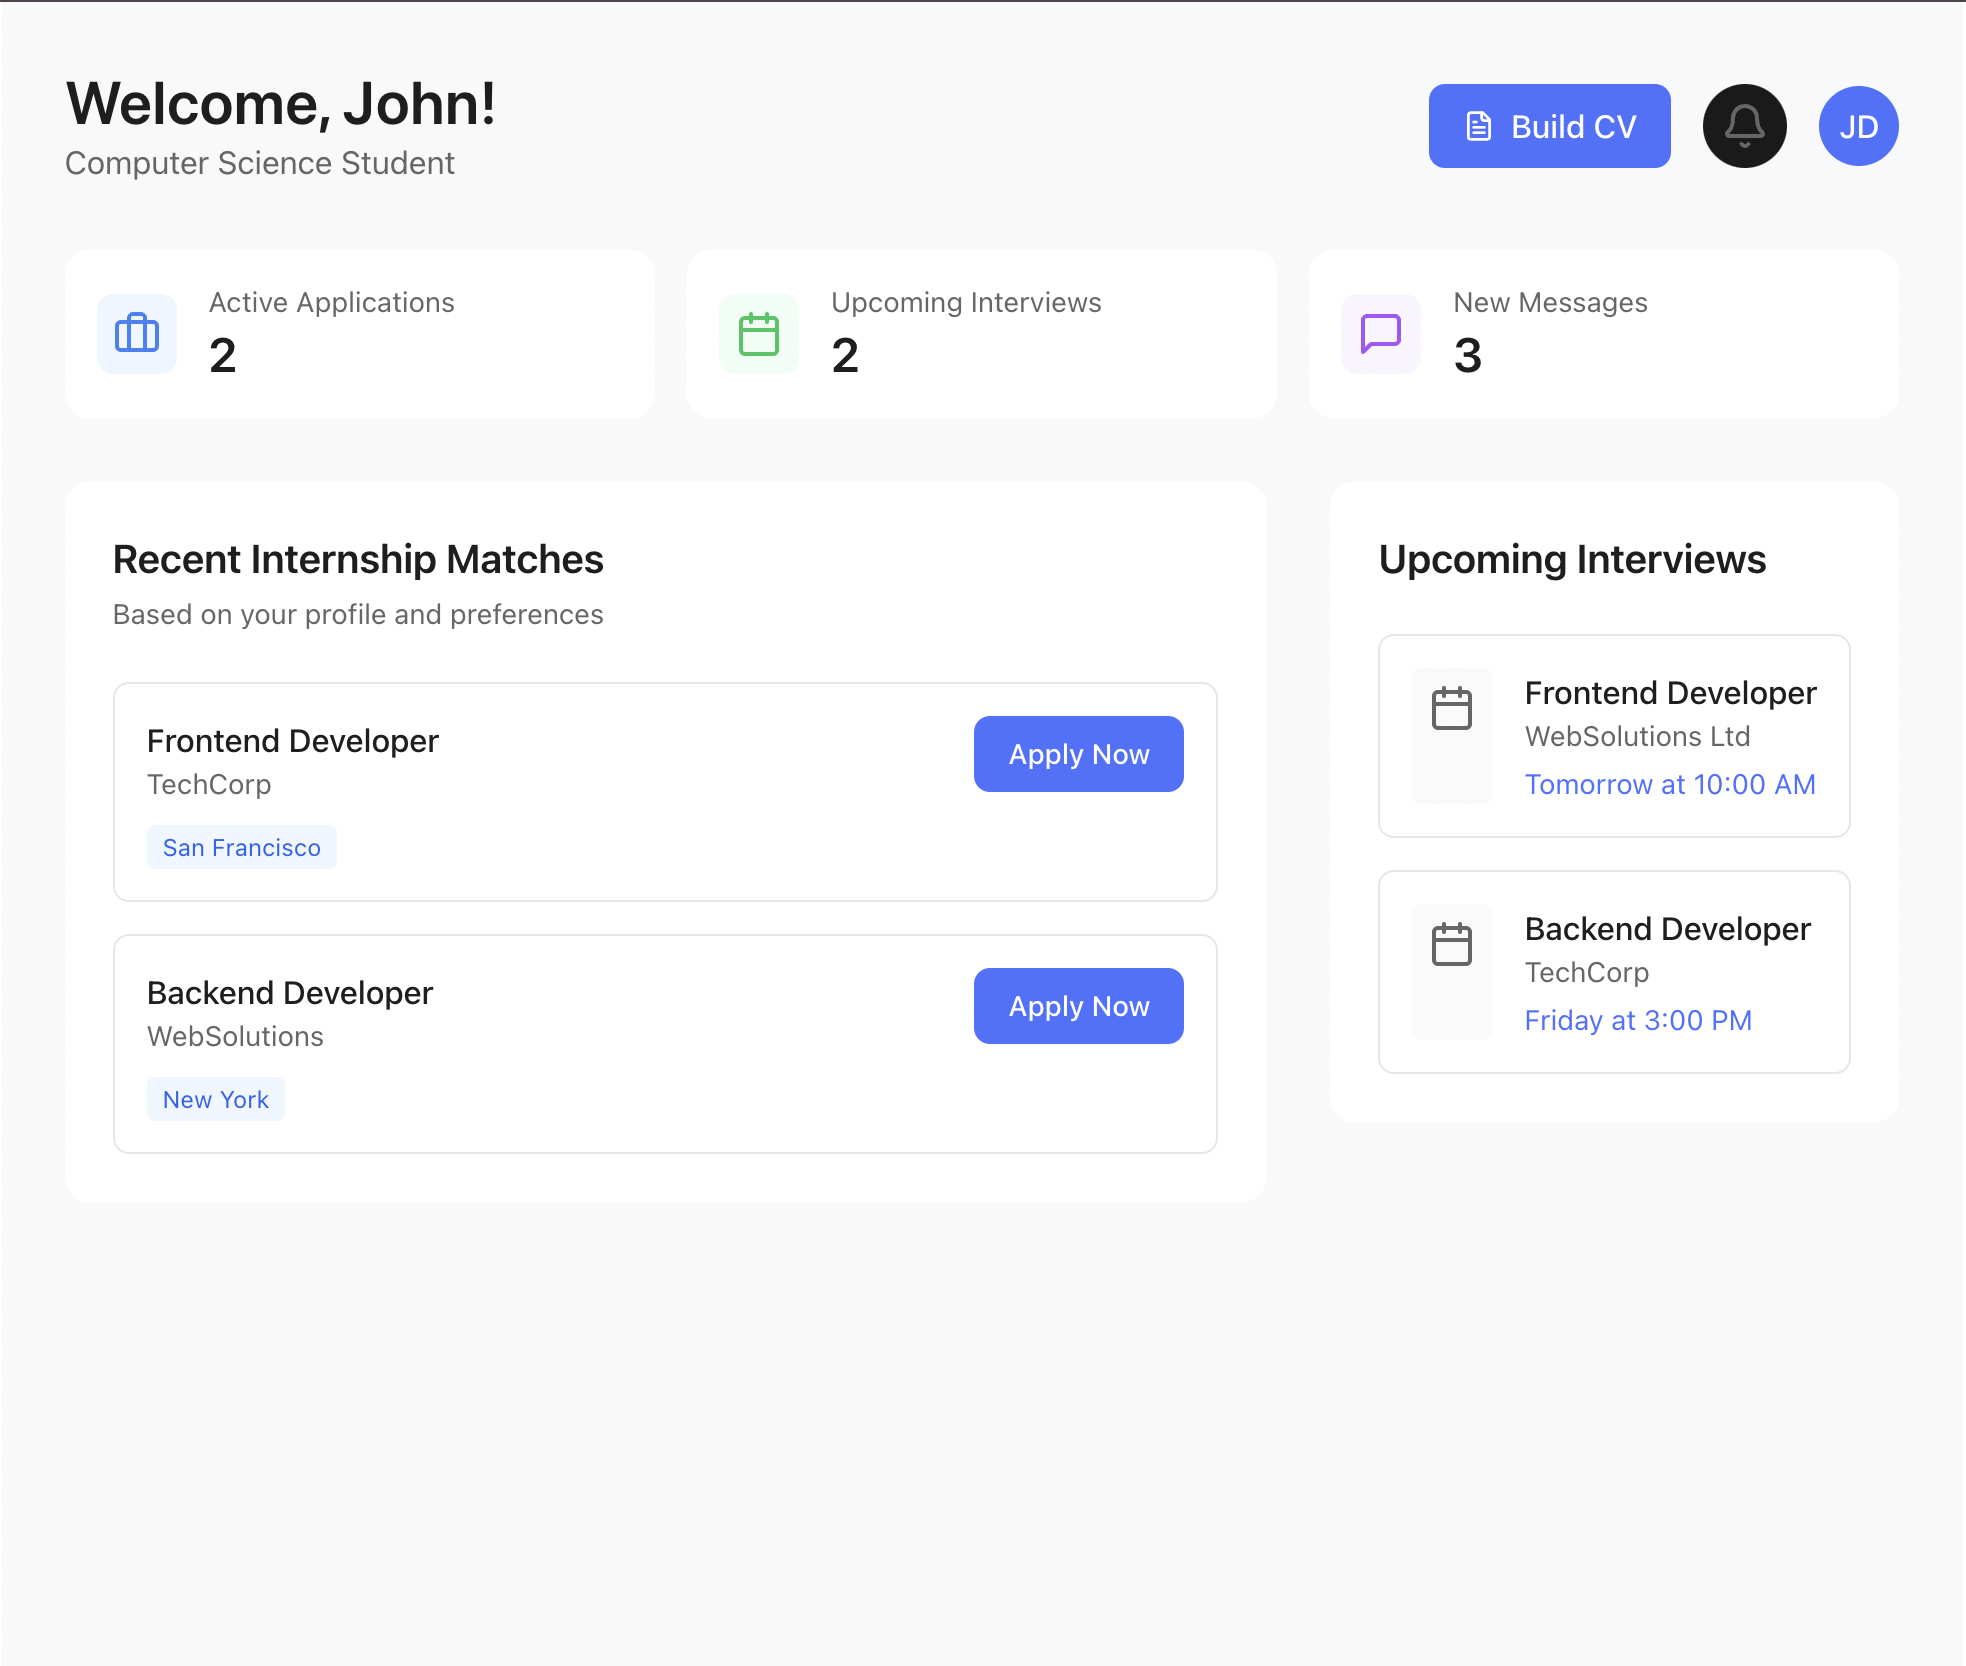
\includegraphics[width=0.82\linewidth]{JhaBhatiaSharma/imagesDD/StudentDashboard.png}
        \caption{Student Dashboard}
        \label{fig:studentDashboard}
    \end{center}
\end{figure}

The \textbf{Student Dashboard} provides a customized and streamlined interface to help students effectively manage their internship applications and search processes. Key features include:
\begin{enumerate}
    \item \textbf{Overview:} Displays key metrics such as Active Applications, Upcoming Interviews, and New Messages.
    \item \textbf{Build CV:} A button to access resume-building resources.
    \item \textbf{Recent Internship Matches:} Shows internship opportunities tailored to the student's profile and preferences, including roles like Frontend Developer and Backend Developer, with company names, locations, and an \textbf{Apply Now} button for quick action.
    \item \textbf{Upcoming Interviews:} Displays scheduled interviews with information about the position, employer, and time.
\end{enumerate}

The layout emphasizes accessibility and relevance, ensuring students can quickly find and act on the most important information to enhance their internship experience.

\subsection{UI6. Build CV}
\label{subsec:build_cv_ui}%

\begin{figure}[H]
    \begin{center}
        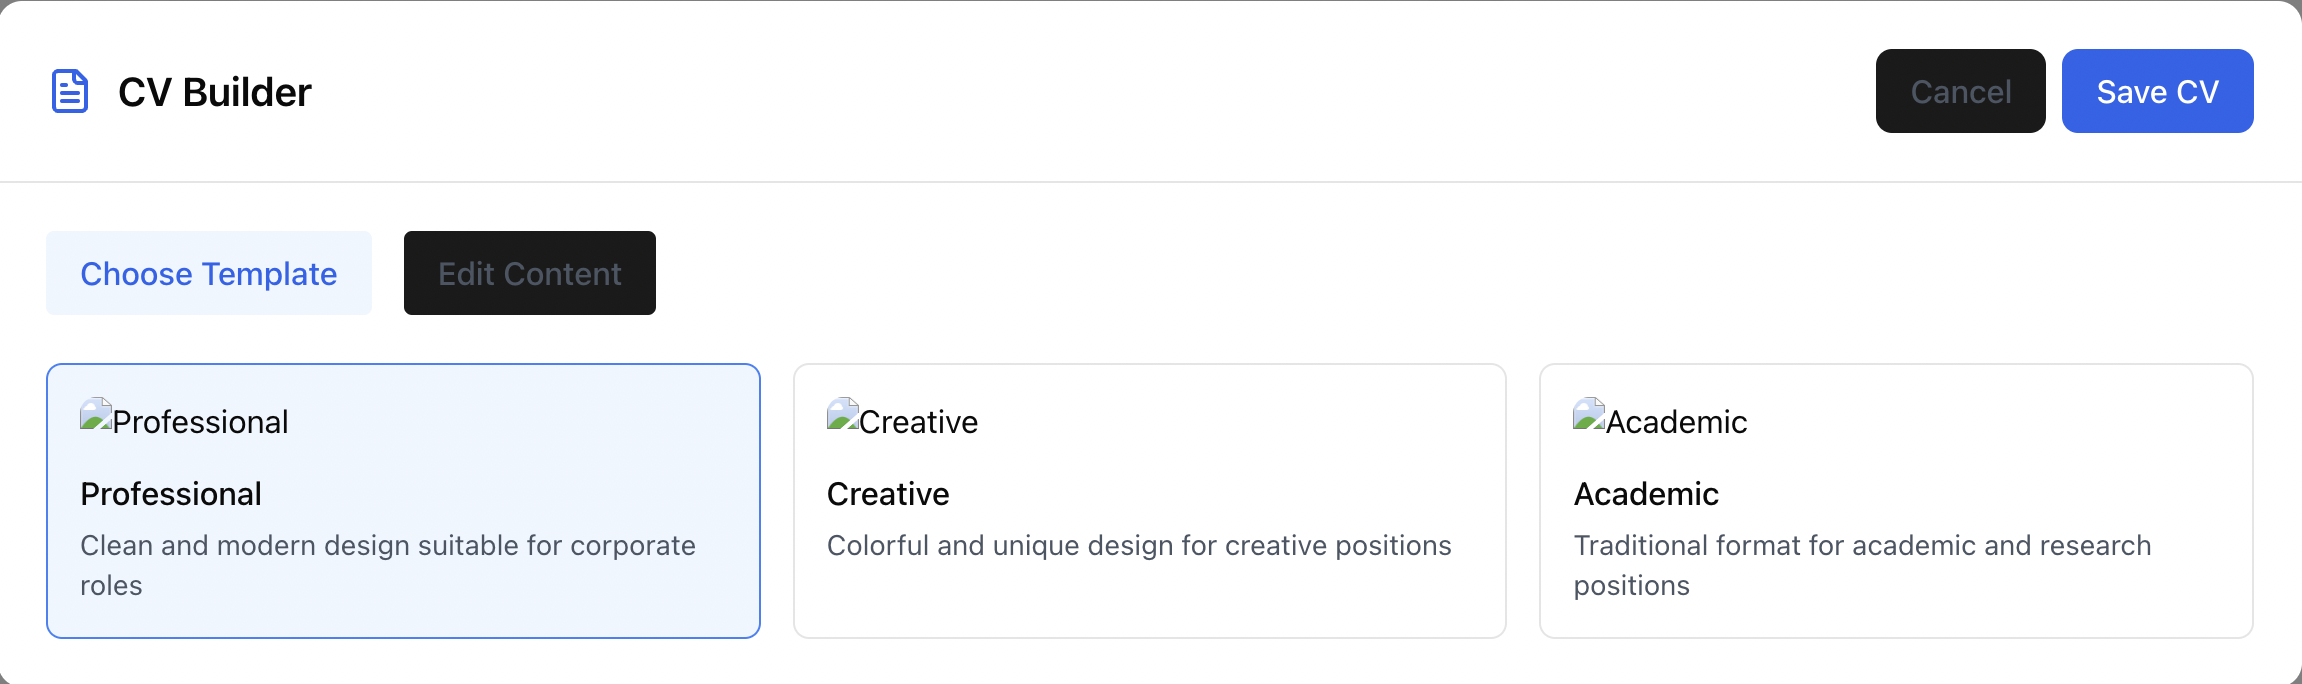
\includegraphics[width=0.82\linewidth]{JhaBhatiaSharma/imagesDD/BuildCV.png}
        \caption{Build CV}
        \label{fig:BuildCV}
    \end{center}
\end{figure}

The \textbf{CV Builder} interface provides a simplified and well-structured layout that enables users to create and modify resumes. The interface includes two primary steps:
\begin{enumerate}
    \item \textbf{Choose Template:} Users can select from three options—Professional, Creative, and Academic—each with a description to help them choose the best format based on their career goals and the type of position they are targeting.
    \item \textbf{Edit Content:} Users can input their personal information, skills, education, and work experience to customize their resume.
\end{enumerate}

Users can \textbf{Cancel} changes or \textbf{Save CV} to finalize their resume using buttons in the upper-right corner. This design ensures users can efficiently create resumes tailored to their professional needs while maintaining simplicity and clarity throughout the process.

\subsection{UI7. Messaging System}
\label{subsec:messaging_system_ui}%

\begin{figure}[H]
    \begin{center}
        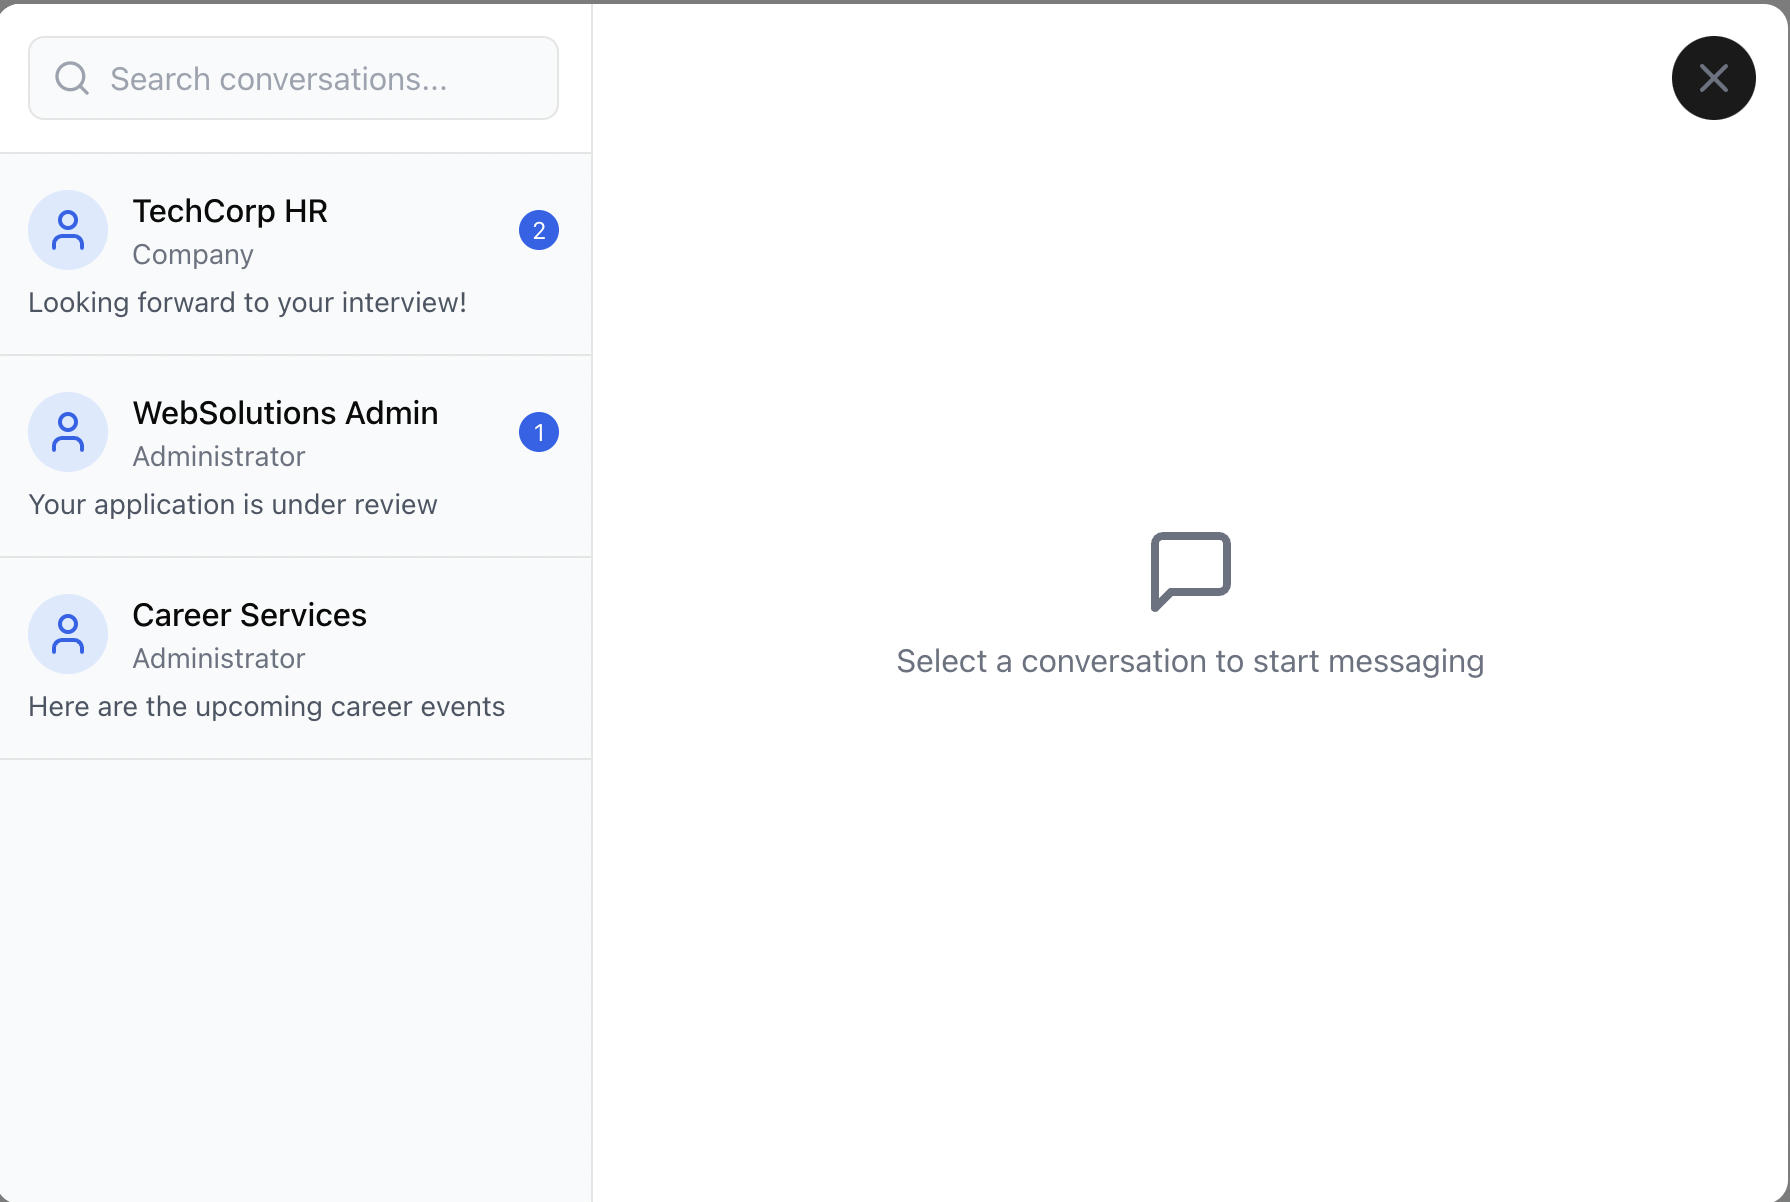
\includegraphics[width=0.82\linewidth]{JhaBhatiaSharma/imagesDD/MessagingSystem.png}
        \caption{Messaging System}
        \label{fig:messagingSystme}
    \end{center}
\end{figure}

The \textbf{Messaging System} interface enables users to have seamless conversations with various stakeholders on the InternHub – Students \& Companies (S\&C) platform. Key features include:
\begin{enumerate}
    \item \textbf{Conversation List:} Arranged on the left side, showing ongoing discussions with details like contact name, role (e.g., Company, Administrator), and a summary of the most recent message. Blue badges indicate the number of unread messages.
    \item \textbf{Chat Panel:} The right panel displays the selected conversation. Users can view and send messages here. If no conversation is selected, a placeholder prompts the user to choose one.
    \item \textbf{Search Bar:} Positioned at the top of the conversation list, enabling users to search for specific discussions.
\end{enumerate}

This split-pane design ensures users can easily navigate their conversations and focus on ongoing chats without interruptions. The interface supports real-time updates, facilitating efficient communication and collaboration between administrators, businesses, and students.

